\section{Implications for the optimization of \acs{WCA}}

In this section, we will discuss the implications of the methodology for the optimization of \gls{WCA} applications, in particular when employing the experimental results and the improved model of human timings discussed in \cref{sec:extendingmethodology}.
The discussion presented here is a summarized version of what \cref{paper:olguinmunoz2023realistic} exposes.

\todo[inline]{Do we need more experiments?}
\todo[inline]{Include discussions on the metrics here (grab inspiration from EdgeDroid2 paper.)}

\subsection{Implications with respect to task completion times}

The term \emph{task completion time}, in the context of \gls{WCA}, will refer to the time it takes a user to work their way through the task presented by an assistant application.
In \cref{paper:olguinmunoz2023realistic} we refer interchangeably to task completion times as application lifetimes.
This metric directly relates to system resource and energy consumption --- longer task completion times mean that the system is occupied for longer and thus uses more resources.
It thus presents a relatively straightforward yet interesting starting point for the study of the implications of the model on the optimization of \gls{WCA} systems.

\begin{figure}
    \centering
    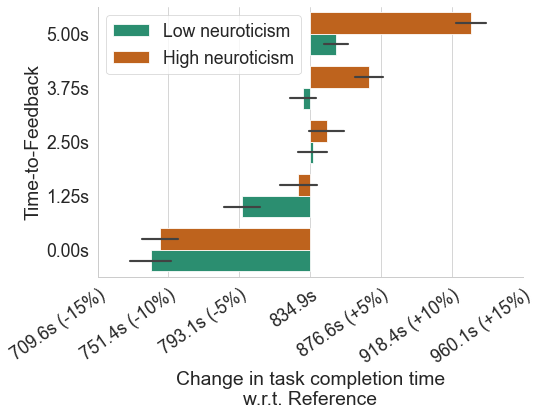
\includegraphics[height=13em]{Figs/2023EdgeDroid2/task_durations_diff}
    \caption{Difference in task completion times of the realistic model with respect to the reference baseline.
    Geometric averages over \num{10} over ten total repetitions per configuration.}\label{fig:taskcompletiontimesdiff}
\end{figure}

The main question we aim to ask relates to the consequences of using our model of human timing behaviors versus using a less realistic approximation.
Specifically, we aim to quantify the difference in task completion times when using the realistic model compared to a baseline which does not take into consideration higher order effects on execution times.
In \cref{fig:taskcompletiontimesdiff} we present the results of an experimental exploration of this difference.
We compare the total task durations of emulated \num{45}-step tasks using the EdgeDroid benchmarking tool with the improved model of human behavior to a baseline model.
Our reference baseline corresponds here to a first order approximation to empirical execution time modeling, using an \gls{exGaussian} distribution fitted to \emph{all} the data points from \cref{paper:olguinmunoz2021impact} (without any grouping) which is randomly sampled to obtain execution time values.
We perform this experiment on the edge computing testbed discussed in \cref{sec:testbed};
for simplicity and to magnify the effects of latency, in this setup we use an \acs{IEEE} \num{802.11}b/g physical layer.

These results show clear and significant differences in task durations between the realistic model and the baseline, with a reduction of up to \SI{11}{\percent} at low levels of resource contention for both levels of neuroticism.
At higher degrees of resource contention, the high neuroticism parameterization also results in task durations more than \SI{8}{\percent} longer than the baseline.

\todo[inline]{Briefly discuss implications of the above?}

\subsection{Implications with respect to number of samples per step}

In the present section and the following we briefly discuss the implications of our methodology on the optimization potential of number of samples and energy consumption per step, respectively.
Both these analyses depend on an understanding of the tradeoffs between resource consumption and responsiveness in \gls{WCA};
fewer samples per step translates into longer sampling periods, and lower energy consumption tends to be made possible by processing fewer bits of data per step.
As such, we employ in these sections an optimization framework for the optimization of said trade-offs based primarily upon the work of Moothedath et al.~\cite{moothedath2021energy,moothedath2022energy1,moothedath2022energy2}.
We note that objective metrics relating to sampling and the responsiveness of a \gls{WCA} system will present itself as a linear combination of the number of expected samples and expected wait time per step plus some constant term:
\begin{align}
    \mathcal{E} = \alpha\mathbb{E}[\mathcal{S}] + \beta\mathbb{E}[\mathcal{W}] + C\label{eq:genericopt}
\end{align}
The above objective function is generic, and can be adapted to any metric which relates to the sampling and responsiveness of \gls{WCA} by modifying the factors \ensuremath{\alpha}, \ensuremath{\beta}, and \ensuremath{C}.

For the analyses in this subsection and \cref{ssec:implications:energy}, we use the solution
\begin{align}
    t_n = \left( 3\sigma\sqrt {\frac{\alpha}{2\beta}} \right)^{\frac{2}{3}} n^{\frac{2}{3}}
\end{align}
where \ensuremath{t_n} once again corresponds to the \ensuremath{n}-th sampling instant in a step.
Note that any positive real value is valid for \ensuremath{\frac{\alpha}{2\beta}}.
This ratio controls the optimization criteria --- as it goes to infinity, the criteria changes from minimizing wait time (i.e.\ maximizing responsiveness) to minimizing the number of samples per step (i.e.\ minimizing energy consumption).

The full derivation and explanation of this framework is out of the scope of this summary.
Please refer to \cref{paper:olguinmunoz2023realistic} and its appendix for a detailed discussion on this optimization approach.
\todo{Include ref to section?}

\medskip





\subsection{Implications with respect to raw energy consumption}\label{ssec:implications:energy}
